\documentclass[10pt]{beamer}

%\usetheme[progressbar=frametitle]{metropolis}
\usecolortheme{spruce}
\usepackage{appendixnumberbeamer}

\usepackage{booktabs}
\usepackage[scale=2]{ccicons}

\usepackage{filecontents}
\usepackage[backend=biber,sorting=none,url=false,doi=false,isbn=false,style=alphabetic]{biblatex}
\addbibresource{uni22.bib}
\usepackage{pgfplots}
\usepgfplotslibrary{dateplot}
\pgfplotsset{compat=1.16}

\usepackage{tikz}
\usetikzlibrary{calc}
\newcommand{\tikzmark}[1]{\tikz[overlay,remember picture] \node (#1) {};}

\usepackage{xspace}
\usepackage{physics}
% \newcommand{\themename}{\textbf{\textsc{metropolis}}\xspace}

\usepackage{hyperref}
\pdfstringdefDisableCommands{%
\def\translate#1{#1}%
}

\newcommand{\mcw}{\mathcal{W}}
\newcommand{\mcf}{\mathcal{F}}
\newcommand{\mcs}{\mathcal{S}}


\title{Thermodynamic Cost of Quantum Information}
% \subtitle{}
% \date{\today}
\date{26th October 2022}
\author{Etienne Springer}
\institute{Institute for Theoretical Physics I}

\begin{document}

\maketitle

\begin{frame}{Table of contents}
    \setbeamertemplate{section in toc}[sections numbered]
    \tableofcontents[hideallsubsections]
\end{frame}

\section[Theoretical Basics]{Theoretical Basics}

\begin{frame}{Basic Notions of Information Theory}
    \begin{minipage}[t]{.4\textwidth}
        classical quantities
        \begin{align*}
            F(p_x, q_x) &\equiv \sum\limits_x \sqrt{p_xq_x}\\
            S[p_x] &\equiv - \sum\limits_x p_x \ln(p_x) \\
            \mathcal{D}[p_x\mid\mid q_x] &\equiv \sum\limits_x p_x\ln(\frac{p_x}{q_x})
        \end{align*}
    \end{minipage}
    \begin{minipage}[t]{.5\textwidth}
        quantum analogues
        \begin{align*}
            F(\rho,\sigma) &\equiv \Tr[\sqrt{\sqrt{\rho}\sigma\sqrt{\rho}}]\\
            S(\rho) &\equiv -\Trace[\rho\ln(\rho)] \\
            S(\rho\mid\mid\sigma) \equiv \Trace[\rho\ln(\rho)] - \Trace[\rho\ln(\sigma)]
        \end{align*}
    \end{minipage}
    %\begin{itemize}
    %    \item Shannon? \footfullcite{BA_HS_nielsenchuang}
    %    \item KLD?
    %    \item Fidelity?
    %\end{itemize}
\end{frame}

\begin{frame}{Pendry's inequality}
    \begin{itemize}
        \item komplette herleitung hier? \cite{BA_Pendry_1983}
    \end{itemize}
\end{frame}

\begin{frame}{The model system}
    \begin{itemize}
        \item hier $XY$ Spinchain
        \item auch: definition von $\dot{I}^2$ und $\dot{E}$
    \end{itemize}
\end{frame}

\begin{frame}{Correlations}
    \begin{itemize}
        \item correlations?
    \end{itemize}
\end{frame}

\section[Numerical Results]{Numerical Results}

\subsection{uncorrelated}

\begin{frame}{uncorrelated}
    \begin{itemize}
        \item hom/longrange/perfect transfer?
        \item which one, all of them?asdf
    \end{itemize}
\end{frame}

%\begin{frame}{entangled}
%    Bell States:
%    \begin{align}
%        \ket{\beta_{00}} &= \frac{\ket{00} +\ket{11}}{\sqrt{2}},\\
%        \ket{\beta_{01}} &= \frac{\ket{01} -\ket{10}}{\sqrt{2}},\\
%        \ket{\beta_{10}} &= \frac{\ket{00} +\ket{11}}{\sqrt{2}}, \qq{and}\\
%        \ket{\beta_{11}} &= \frac{\ket{01} -\ket{10}}{\sqrt{2}}.
%    \end{align}
%\end{frame}

\begin{frame}{Quantum Correlations}
    \begin{align}\label{eq:kaonans-corr}
        \chi = -i\alpha(\sigma^+_k \sigma^-_{k+1} - \sigma^-_k \sigma^+_{k+1}),
    \end{align}
    vielleicht auxilliary slide mit quantum discord
\end{frame}

\begin{frame}{hm?}
    \begin{itemize}
        \item pos/temp dependence?
        \item corr dependence?
        \item which of the pos/temp/corr dependence?
    \end{itemize}
\end{frame}

\begin{frame}{Bound on information flow with correlations}
    am ende nur die mit dashed line old bound?
\end{frame}

\section[Conclusion and Outlook]{Conclusion}

\begin{frame}{Conclusion}
    \begin{itemize}
        \item Pendry
        \item Pendry doesnt hold for quantum correlations
        \item new pendry:
    \end{itemize}
    ...
\end{frame}

\appendix

\begin{frame}
    \printbibliography    
\end{frame}

\section*{auxiliary slides}

\begin{frame}{welche}
    \begin{itemize}
        \item quantum discord?
        \item bell states?
        \item BA appendix?
    \end{itemize}
\end{frame}

\begin{frame}{entangled}
    \begin{figure}[H]
        \centering
        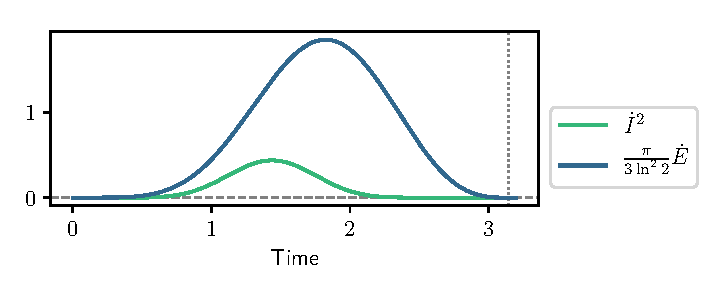
\includegraphics[width=\textwidth]{alltheplots/bell/pendry_grey_lines.pdf}
        \caption{Energy flow and information flow of qubit $5$ for 
        initially entangled qubits $1$ and $2$.
        That is, $\rho_{12} = \dyad{\beta_{11}}$ with Bell state $\ket{\beta_{11}} = \left(\ket{01}-\ket{10}\right)/\sqrt{2}$.
        The dotted vertical line indicates $t=\pi$, which is the time of state inversion, i.e. where the dynamics reverse,
        given by the interaction.
        The dashed horizontal line denotes $0$, and is drawn in as visual aids.}
        \label{fig:bell_pendry}
    \end{figure}
\end{frame}

\end{document}
